
\section{Friday}\index{week7_Friday_lecture}
\subsection{Review}
\begin{itemize}
\item
\emph{Diagonalization: }Suppose the matrix $\bm A\in\mathbb{R}^{n\times n}$ is diagonalizable, it's equivalent to say it has $n$ independent eigenvectors. These $n$ independent eigenvectors form a basis for $\mathbb{R}^n$. $(*)$
\item
If all \textit{eigenvalues of $\bm A$ are distinct}, then $(*)$ holds.
\end{itemize}
\subsection{Fibonacci Numbers}
We show a famous example, where the eigenvalues tell how to find the formula for Fibonacci Numbers.
\paragraph{Every new Fibonacci number come from two previous ones}
\begin{align*}
\text{\emph{Fibonacci Number: }}&0,1,1,2,3,5,8,13,\dots\\
\text{\emph{Fibonacci Equation: }}&\bm F_{k+2}=\bm F_{k+1}+\bm F_{k},\quad\bm F_0=0,\bm F_1=1.
\end{align*}
\paragraph{How to compute $\bm F_{100}$ without computing $\bm F_2$ to $\bm F_{99}$?}
The key is to begin with a matrix equation $\bm u_{k+1}=\bm A\bm u_k$. We put two Fibonacci number into a vector $\bm u_k$, then you will see the matrix $\bm A$:

Define $\bm u_k:=\begin{bmatrix}
\bm F_{k+1}\\\bm F_k
\end{bmatrix}.$ The rule $\left\{
\begin{aligned}
\bm F_{k+2}&=\bm F_{k+1}+\bm F_{k}\\\bm F_{0}&=0, \bm F_1=1
\end{aligned}\right.$ implies that
\[
\begin{array}{ll}
\bm u_{k+1}=\begin{bmatrix}
1&1\\1&0
\end{bmatrix}\bm u_{k},
&
\bm u_0=\begin{bmatrix}
1\\0
\end{bmatrix}
\end{array}.
\]

Every step we mutliply $\bm u_0$ by $\bm A$. After 100 steps we obtain $\bm u_{100}=\bm A^{100}\bm u_0$:
\[
\bm u_{100}=\begin{bmatrix}
\bm F_{101}\\\bm F_{100}
\end{bmatrix}=\bm A^{100}\bm u_0=\bm A^{100}\begin{bmatrix}
1\\0
\end{bmatrix}.
\]

How to compute the matrix powers $\bm A^{100}$? Diagonalizing $\bm A$ is possible. It's easy to verify that the matrix $\bm A=\begin{bmatrix}
1&1\\1&0
\end{bmatrix}$ can be decomposed into $
\bm A=\bm S\bm D\bm S^{-1}
$, where
\[
\begin{array}{ll}
\bm D=\diag(\lambda_1,\lambda_2),
&
\bm S=\begin{bmatrix}
\lambda_1&\lambda_2\\1&1
\end{bmatrix},\\
\left(\lambda_1,\begin{bmatrix}
\lambda_1\\1
\end{bmatrix}\right),
&
\left(\lambda_2,\begin{bmatrix}
\lambda_2\\1
\end{bmatrix}\right)
\mbox{ are two eigen-pairs of $\bm A$},
\end{array}
\]
with $\lambda_1=\frac{1+\sqrt{5}}{2},\lambda_2=\frac{1-\sqrt{5}}{2}.$

If follows that $\bm A^{100}=\bm S\bm D^{100}\bm S^{-1}$. Hence we can compute $\bm u_{100}$:
\begin{align*}
\bm u_{100}&=\bm A^{100}\bm u_0=\bm S\bm D^{100}\bm S^{-1}\bm u_0=\bm S\begin{pmatrix}
\lambda_1^{100}&\\&\lambda_2^{100}
\end{pmatrix}\bm S^{-1}\bm u_0
\\&=\begin{bmatrix}
\lambda_1&\lambda_2\\1&1
\end{bmatrix}\begin{pmatrix}
\lambda_1^{100}&\\&\lambda_2^{100}
\end{pmatrix}\begin{bmatrix}
\lambda_1&\lambda_2\\1&1
\end{bmatrix}^{-1}\begin{bmatrix}
1\\0
\end{bmatrix}=\begin{bmatrix}
\bm F_{101}\\\bm F_{100}
\end{bmatrix}
\end{align*}

After messy computation, we obtain $\bm F_{100}$:
\[
\bm F_{100}=\frac{1}{\sqrt{5}}\left[\lambda_1^{100}-\lambda_2^{100}\right]
=\frac{1}{\sqrt{5}}\left[\left(\frac{1+\sqrt{5}}{2}\right)^{100}-\left(\frac{1-\sqrt{5}}{2}\right)^{100}\right]
\]
\paragraph{Another way to compute $\bm F_{100}$}

As $\bm u_{k+1} = \bm A\bm u_k$, we apply a trick to simplify $\bm u_0$ at first:

We set $\bm S=\begin{bmatrix}
\bm x_1&\bm x_2
\end{bmatrix}$, where $\bm x_1=\begin{bmatrix}
\lambda_1\\1
\end{bmatrix},\bm x_2=\begin{bmatrix}
\lambda_2\\1
\end{bmatrix}.$
It follows that
\[
\bm u_0=\begin{bmatrix}
1\\0
\end{bmatrix}
=\frac{1}{\lambda_1-\lambda_2}\left(\begin{bmatrix}
\lambda_1\\1
\end{bmatrix}-\begin{bmatrix}
\lambda_2\\1
\end{bmatrix}\right)\implies
\bm u_0=\frac{\bm x_1-\bm x_2}{\lambda_1-\lambda_2}
\]
Then we multiply $\bm u_{0}$ by $\bm A^{100}$ to get $\bm u_{100}$:
\begin{align*}
\bm u_{100}&=\bm A^{100}\bm u_0=\frac{\bm A^{100}\bm x_1-\bm A^{100}\bm x_2}{\lambda_1-\lambda_2}\\
&=\frac{\bm A^{99}(\bm A\bm x_1)-\bm A^{99}(\bm A\bm x_2)}{\lambda_1-\lambda_2}=\frac{\lambda_1\bm A^{99}\bm x_1-\lambda_2\bm A^{99}\bm x_2}{\lambda_1-\lambda_2}=\frac{\lambda_1^2\bm A^{98}\bm x_1-\lambda_2^2\bm A^{98}\bm x_2}{\lambda_1-\lambda_2}=\dots\\
&=\frac{\lambda_1^{100}\bm x_1-\lambda_2^{100}\bm x_2}{\lambda_1-\lambda_2}
\end{align*}
After simplification, finally we obtain the same result.
\subsection{Imaginary Eigenvalues}
The eigenvalues might not be real numbers sometimes.
\begin{example}\label{Exp:7:6}
Consider the rotation matrix given by $\bm K=\begin{bmatrix}
0&-1\\1&0
\end{bmatrix}$. It rotates our vector by $90\degree$:
\[
\bm K\begin{pmatrix}
\cos\theta\\\sin\theta
\end{pmatrix}=\begin{pmatrix}
-\sin\theta\\\cos\theta
\end{pmatrix}.
\]
\begin{figure}[H]
\centering
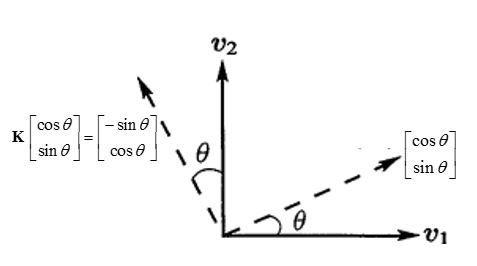
\includegraphics[width=10cm]{week6/rotation}
\caption{Rotate a vector by $90\degree$.}
\end{figure}
This rotation matrix exists eigenvector and eigenvalue, i.e., $\exists\bm v\ne\bm 0$ and $\lambda$ s.t. 
\[\bm K\bm v=\lambda\bm v.\] 
However, the equation above means the rotaion matrix doesn't change the direction of $\bm v$. In geometric meaning it rotates vector $\bm v$ by $90\degree$. It seems a contradiction. \emph{This phenomenon will not happen unless we go to imaginary eigenvectors.} Let's compute eigenvalues and eigenvectors for $\bm K$ first:
\[
P_{\bm K}(\lambda)=\begin{vmatrix}
\lambda&1\\-1&\lambda\end{vmatrix}
=\lambda^2+1
\implies
\lambda_1=i,\quad\lambda_2=-i.
\]
\begin{align*}
(\lambda_1\bm I-\bm K)\bm x&=\begin{pmatrix}
i&1\\-1&i
\end{pmatrix}\begin{pmatrix}
x_1\\x_2
\end{pmatrix}=\bm 0\implies\bm x=\alpha\begin{pmatrix}
1\\-i
\end{pmatrix}.\\
(\lambda_2\bm I-\bm K)\bm x&=\begin{pmatrix}
-i&1\\-1&-i
\end{pmatrix}\begin{pmatrix}
x_1\\x_2
\end{pmatrix}=\bm 0\implies\bm x=\beta\begin{pmatrix}
1\\i
\end{pmatrix}.
\end{align*}
Moverover, we can diagonalize $\bm K$:
\[
\begin{array}{ll}
\bm D=\bm S^{-1}\bm K\bm S=\begin{pmatrix}
i&\\&-i
\end{pmatrix}
&
\mbox{ where }\bm S=\begin{bmatrix}
1&1\\-i&i
\end{bmatrix}.
\end{array}
\]
\end{example}
\begin{remark}
For motion in vector space, eigenvalues are ``speed''
 and eigenvectors are ``directions'' under the basis $\bm S=\begin{bmatrix}
\bm x_1&\bm x_2&\dots&\bm x_n
\end{bmatrix}$.
\[
\bm v=c_1\bm x_1+\dots+c_n\bm x_n
\xLongrightarrow{\text{postmultiply $\bm A$}}\bm{Av}=c_1\lambda_1\bm x_1+\dots+c_n\lambda_n\bm x_n.
\]
\[
\begin{pmatrix}
c_1&\dots&c_n
\end{pmatrix}
\xLongrightarrow{\text{rightmultiply $\bm D=\diag(\lambda_1,\dots,\lambda_n)$}}
\begin{pmatrix}c_1\lambda_1&\dots&c_n\lambda_n
\end{pmatrix}.
\]
\end{remark}
\subsection{Complex Numbers and vectors}
From Example(\ref{Exp:7:6}) we can see that even for a real matrix, its eigenvaluesmay be complex numbers. 
\begin{definition}[Complex Numbers]
A complex number $\bm x\in\mathbb{C}$ could be written as 
\[
\bm x=a+bi,
\] 
where $i^2=-1$.

Its \emph{complex conjugate} is defined as $\bm{\bar x}=a-bi$.

Its \emph{modulus} is defined as $|\bm x|=\sqrt{a^2+b^2}=\sqrt{\bm x\bm{\bar x}}.$
\end{definition}
\begin{figure}[H]
\centering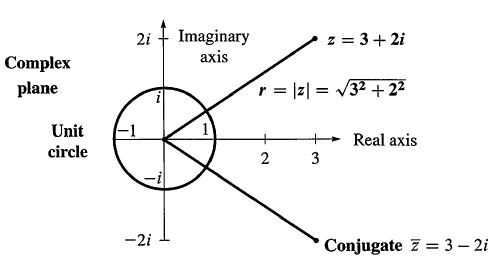
\includegraphics{week6/complex}
\caption{The number $z=a+bi$ corrsponds to the vector 
$(a,b)$.}
\end{figure}
\begin{definition}[Length (norm) for complex]
Given a complex-valued $n$-dimension column vector
\[
z=\begin{bmatrix}
z_1\\z_2\\\vdots\\z_n
\end{bmatrix}\in\mathbb{C}^n,
\] 
its \emph{length (norm)} is defined as
\[
\|z\|=\sqrt{|z_1|^2+|z_2|^2+\dots+|z_n|^2}=\sqrt{\inp{z}{z}}=\sqrt{z_1\bar z_1+z_2\bar z_2+\dots+z_n\bar z_n}.
\]
\end{definition}

Before introducing the definition of inner product for complex, let's introduce the \emph{Hermitian transpose} for a complex-valued vector:
\begin{definition}[Hermitian transpose]
Given $\bm z\in\mathbb{C}^n$, we use $\bm z\Her$ denote its \emph{Hermitian transpose}:
\[
\bm z=\begin{bmatrix}
z_1\\\vdots\\z_n
\end{bmatrix}\implies
\bm z\Her=\bm{\bar z}\trans=\begin{bmatrix}
\bar z_1&\dots&\bar z_n
\end{bmatrix}.
\]
where $\bar z_i$ denotes the complex conjugate of $z_i$.
\end{definition}
\begin{definition}[Inner product]
The inner product of complex-valued vectors $\bm z$ and $\bm w$ is defined as
\[
\inp{\bm z}{\bm w}=\bm w\Her\bm z=\begin{bmatrix}
\bm{\bar w_1}&\dots&\bm{\bar w_n}
\end{bmatrix}\begin{bmatrix}
\bm{z_1}\\\vdots\\\bm{z_n}
\end{bmatrix}=\bm{\bar w_1}\bm{z_1}+\dots+\bm{\bar w_n}\bm{z_n}.
\]
\end{definition}
\begin{remark}
Note that with complex-valued vectors, $\bm w\Her\bm z$ is different from $\bm z\Her\bm w$. \emph{The order of the vectors is now important!} In fact, $\bm z\Her\bm w=\bm{\bar z_1}\bm{w_1}+\dots+\bm{\bar z_n}\bm{w_n}$ is the complex conjugate of $\bm w\Her\bm z$.
\end{remark}
\begin{definition}[Orthogonal]
Two complex-valued vectors are \textit{orthogonal} if their \emph{inner product} is zero:
\[
\bm z\perp\bm w\implies
\inp{\bm z}{\bm w}=\bm w\Her\bm z=0
\]
\end{definition}
\begin{example}
Given complex-valued vectors
$\bm z=\begin{pmatrix}
1\\i
\end{pmatrix}$ and $\bm w=\begin{pmatrix}
-i\\1
\end{pmatrix}$,
although we have $\bm z\trans\bm w=0$, these two vectors are not perpendicular.

This is because $\inp{\bm z}{\bm w}=\bm w\Her\bm z=\begin{bmatrix}
i&1
\end{bmatrix}\begin{bmatrix}
1\\i
\end{bmatrix}=2i\ne0.$
\end{example}
\begin{example}
The inner product of $\bm u=\begin{bmatrix}
1\\i
\end{bmatrix}$ and $\bm v=\begin{bmatrix}
i\\1
\end{bmatrix}$ is 
\[
\inp{\bm u}{\bm v}=\begin{bmatrix}
-i&1
\end{bmatrix}\begin{bmatrix}
1\\i
\end{bmatrix}=0.
\]
Although these vectors $(1,i)$ and $(i,1)$ don't look  perpendicular, actually they are!
\end{example}
\begin{proposition}[Conjugate symmetry]\qquad\\
For two vectors $\bm z$ and $\bm w\in\mathbb{C}^{n}$, we have $\overline{\inp{\bm z}{\bm w}}=\inp{\bm w}{\bm z}.$
\end{proposition}
\begin{proof}[Verify:]
\begin{gather*}
\inp{\bm z}{\bm w}=\bm w\Her\bm z=\bm{\bar w}\trans\bm z
=\bm{\bar w_1}\bm{z_1}+\dots+\bm{\bar w_n}\bm{z_n}
\\
\inp{\bm w}{\bm z}=\bm z\Her\bm w=\bm{\bar z}\trans\bm w
=\bm{\bar z_1}\bm{w_1}+\dots+\bm{\bar z_n}\bm{w_n}
\end{gather*}
Since we have $\overline{\bm w\bm v}=\bm{\bar w}\bm{\bar v}$ and $\overline{\bm w+\bm v}=\bm{\bar w}+\bm{\bar v}$, it's easy to find that
\[
\overline{\bm{\bar w_1}\bm{z_1}+\dots+\bm{\bar w_n}\bm{z_n}}
=\bm{w_1}\bm{\bar z_1}+\dots+\bm{w_n}\bm{\bar z_n}.
=\bm{\bar z_1}\bm{w_1}+\dots+\bm{\bar z_n}\bm{w_n}.
\]
Hence $\overline{\inp{\bm z}{\bm w}}=\inp{\bm w}{\bm z}.$
\end{proof}
\begin{proposition}[Sesquilinear]
For two vectors $\bm z$ and $\bm w\in\mathbb{C}^{n}$, we have
\begin{gather}
\inp{\alpha\bm z}{\bm w}=\alpha\inp{\bm z}{\bm w}\\
\inp{\bm z}{\beta\bm w}=\bar\beta\inp{\bm z}{\bm w}\label{eq:16.2}
\end{gather}
for scalars $\alpha$ and $\beta$.
\end{proposition}
\begin{proof}[Verify:]
\begin{align*}
\inp{\alpha\bm z}{\bm w}&=\bm w\Her(\alpha\bm z)\\&=\alpha(\bm w\Her\bm z)\\&=\alpha\inp{\bm z}{\bm w}.
\end{align*}
To show the equation (\ref{eq:16.2}), due to the conjugate symmetry, we derive
\[
\inp{\bm z}{\beta\bm w}=\overline{\inp{\beta\bm w}{\bm z}}
\]
Since $\inp{\beta\bm w}{\bm z}=\beta\inp{\bm w}{\bm z}=\beta\overline{\inp{\bm z}{\bm w}}$, we obtain
\[
\inp{\bm z}{\beta\bm w}=\overline{\beta\overline{\inp{\bm z}{\bm w}}}=\bar\beta\inp{\bm z}{\bm w}.
\]
\end{proof}

\subsubsection{Hermitian transpose for matrix}
Similarly, the \emph{Hermitian transpose} of a complex-valued matrix $\bm A$ is given by
\[
\bm A\Her:=\bar{\bm A}\trans
\]
The rules for Hermitian transpose usually comes from transpose. For example, the Hermitian transpose for matrics has the property
\begin{itemize}
\item
$(\bm A\bm B)\Her=\bm B\Her\bm A\Her.$
\item
$(\bm A\Her)\Her=\bm A$.
\item
$(\bm A+\bm B)\Her=\bm A\Her+\bm B\Her.$
\end{itemize}
The rules for Hermitian transpose of complex-valued vectors might be slightly different from the transpose of real-valued vectors:
\begin{center}
\begin{tabular}{cU}
\hline
  $\mathbb{R}^n$  & $\mathbb{C}^n$ \\
  
$\inp{\bm x}{\bm y}=\bm x\trans\bm y$ &  $\inp{\bm z}{\bm w}=\bm w\Her\bm z$\\

$\bm x\trans\bm y=\bm y\trans\bm x$  & $\bm z\Her\bm w=\overline{\bm w\Her\bm z}$\\

$\|\bm x\|^2=\bm x\trans\bm x$   &   $\|\bm z\|^2=\bm z\Her\bm z$\\

$\bm x\perp\bm y\Longleftrightarrow \bm x\trans\bm y=0$&
$\bm z\perp\bm w\Longleftrightarrow \bm w\Her\bm z=0$\\
\hline
\end{tabular}
\end{center}
\begin{remark}
\textit{What aspects of eigenvalues/eigenvectors are not nice?}
\begin{itemize}
\item
Some matrix are \textit{non-diagonalizable}. (or equivalently, eigenvectors aren't independent.)
\item
Eigenvalues can be \textit{complex} even for a real-valued matrix.
\end{itemize}
\end{remark}
We are curious about what kind of matrix has all real eigenvalues? Let's focus on real-valued matrix first. The answer is the real-valued symmetric matrix.

You should remember the proposition(\ref{real_symmetric}) below carefully, they are very important!
\begin{proposition}\label{real_symmetric}
For a \textit{real symmetric} matrix $\bm A$, 
\begin{itemize}
\item
All eigenvalues are real numbers.
\item
The eigenvectors associated with distinct eigenvalues are orthogonal.
\item
$\bm A$ is diagonalizable. More general, all eigenvectors of $\bm A$ are orthogonal!
\end{itemize}
\end{proposition}
Before the proof, let's introduce a useful formula: $\inp{\bm{Ax}}{\bm y}=\inp{\bm x}{\bm A\Her\bm y}$.\\
\[
\textit{Verify: }\inp{\bm{Ax}}{\bm y}=\bm y\Her\bm{Ax}=(\bm A\Her\bm y)\Her\bm x=\inp{\bm x}{\bm A\Her\bm y}
\]
\begin{proof}
\begin{itemize}
\item
For the first part, given any eigen-pair $(\lambda, \bm x)$, we we obtain
\[
\inp{\bm{Ax}}{\bm x}=\inp{\bm x}{\bm A\Her\bm x}
\]
\begin{itemize}
\item
For the LHS, $\inp{\bm{Ax}}{\bm x}=\inp{\lambda\bm x}{\bm x}=\lambda\inp{\bm x}{\bm x}$.
\item
For the RHS, since $\bm A$ is a real symmetric matrix, we have 
\[
\bm A\Her=\bar{\bm A}\trans=\bm A\trans=\bm A\implies
\inp{\bm x}{\bm A\Her\bm x}=\inp{\bm x}{\bm{Ax}}
\]
Moreover, $\inp{\bm x}{\bm{Ax}}=\inp{\bm x}{\lambda\bm x}=\bar\lambda\inp{\bm x}{\bm x}$. Hence, $\inp{\bm x}{\bm A\Her\bm x}=\bar\lambda\inp{\bm x}{\bm x}.$
\end{itemize}
Finally we have $\lambda\inp{\bm x}{\bm x}=\bar\lambda\inp{\bm x}{\bm x}.$
Since $\bm x\ne\bm 0$, $\inp{\bm x}{\bm x}\ne0.$ Hence $\lambda=\bar\lambda$, i.e, $\lambda$ is real.
\item
For the second part, suppose $\bm x_1$ and $\bm x_2$ are two eigenvectors corresponding to two \emph{distinct} eigenvalues $\lambda_1$ and $\lambda_2$ respectively. Our goal is to show $\bm x_1\perp\bm x_2$. We find that
\[
\inp{\bm A\bm x_1}{\bm x_2}=\inp{\bm x_1}{\bm A\Her\bm x_2}
\]
\begin{itemize}
\item
For LHS, $\inp{\bm A\bm x_1}{\bm x_2}=\inp{\lambda_1\bm x_1}{\bm x_2}=\lambda_1\inp{\bm x_1}{\bm x_2}$.
\item
For RHS, $\inp{\bm x_1}{\bm A\Her\bm x_2}=\inp{\bm x_1}{\bm A\bm x_2}=\inp{\bm x_1}{\lambda_2\bm x_2}=\bar\lambda_2\inp{\bm x_1}{\bm x_2}$. From part one we derive that $\inp{\bm x_1}{\bm A\Her\bm x_2}=\lambda_2\inp{\bm x_1}{\bm x_2}.$
\end{itemize}
Hence $\lambda_1\inp{\bm x_1}{\bm x_2}=\lambda_2\inp{\bm x_1}{\bm x_2}.$\\ Since $\lambda_1\ne\lambda_2$, we obtain $\inp{\bm x_1}{\bm x_2}=0$, i.e., $\bm x_1\perp\bm x_2.$
\item
The proof for the third part is not required.
\end{itemize}
\end{proof}
\subsection{Spectral Theorem}
We have a stronger version of the third part of proposition(\ref{real_symmetric}):
\begin{theorem}[Spectral Theorem]
Any real symmetric matrix $\bm A$ has the factorization \begin{equation}
\bm A=\bm Q\Lambda\bm Q\trans,
\end{equation} where $\Lambda\in\mathbb{R}^{n\x n}$ is diagonal matrix, $\bm Q\in\mathbb{R}^{n\x n}$ is orthogonal.
\end{theorem}
\begin{proof}
From proposition (\ref{real_symmetric}) we know that $\bm A$ is \textit{diagonalizable}, i.e., there exists invertible matrix $\bm Q$ and diagonal matrix $\Lambda$ such that
\[
\bm A=\bm Q\Lambda\bm Q^{-1}
\]

From proposition(\ref{real_symmetric}), since all eigenvalues of $\bm A$ are real, $\Lambda$ is a real matrix.

Since all eigenvectors $\bm x_1,\dots,\bm x_n$ are orthogonal, from proposition(\ref{Pro:7:5}), matrix $\bm Q=\begin{bmatrix}
\bm x_1&\dots&\bm x_n
\end{bmatrix}$,  we imply $\bm Q$ is orthogonal.
\end{proof}
\begin{remark}
\begin{enumerate}
\item
Since $\bm A=\bm Q\Lambda\bm Q\trans=\bm Q\Lambda\bm Q^{-1}$, $\bm A$ could be diagonalized by an orthogonal matrix.
\item
Suppose $\bm Q=\begin{bmatrix}
q_1&\dots&q_n
\end{bmatrix}$, $\Lambda=\diag(\lambda_1,\dots,\lambda_n)$, then $\bm A$ could be rewritten as:
\[
\bm A=
\begin{bmatrix}
q_1&\dots&q_n
\end{bmatrix}\begin{bmatrix}
\lambda_1&&\\&\ddots&\\&&\lambda_n
\end{bmatrix}\begin{bmatrix}
q_1\trans\\\vdots\\q_n\trans
\end{bmatrix}
\]
Or equivalently,
\begin{equation}
\bm A=\lambda_1q_1q_1\trans+\lambda_2q_2q_2\trans+\dots+\lambda_nq_nq_n\trans
\end{equation}
Note that each term $q_iq_i\trans$ is the \emph{projection matrix} for $q_i$. Hence spectral theorem says that a real symmetric matrix is a linear combination of projection matrices.
\end{enumerate}
\end{remark}

\begin{example}
If we write $\bm A$ as a linear combination of projection matrices, we can have a deep understanding for the linear transformation $\bm{Ax}$:
\[
\bm A=\sum_{j=1}^{n}\lambda_jq_jq_j\trans
\implies
\bm{Ax}=\sum_{j=1}^{n}\lambda_jq_jq_j\trans\bm x=
\sum_{j=1}^{n}\lambda_j(q_jq_j\trans\bm x).
\]
For the case $n=2$, it's clear to find that
\[
\bm x=c_1q_1+c_2q_2\implies
\bm{Ax}=\lambda_1c_1q_1+\lambda_2c_2q_2
\]
Showing in graph, we have
\begin{figure}[H]
\centering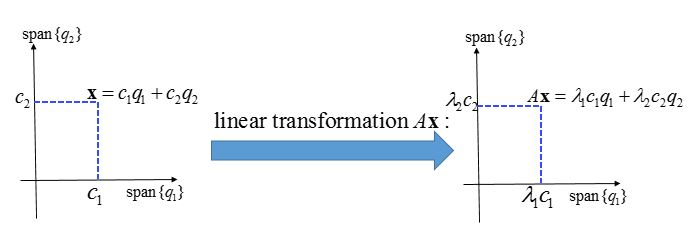
\includegraphics[width=12cm]{week6/spec}
\caption{Linear transformation of $\bm A$.}
\end{figure}
\end{example}
\begin{remark}
The formula \[
\bm A=\sum_{j=1}^{n}\lambda_jq_jq_j\trans\mbox{ or }\bm A=\bm Q\Lambda\bm Q\trans
\] are called the \emph{eigen-decomposition} or \emph{eigenvalue decomposition} of $\bm A$.

$\{\lambda_1,\dots,\lambda_n\}$ are called the \emph{spectum} of $\bm A$.
\end{remark}
Also, we can extend our result from real symmetric matrix into complex-valued.
\subsection{Hermitian matrix}
\begin{definition}[Symmetric and Hermitian]
\begin{itemize}
\item
Recall that a square matrix $\bm A$ is said to be \emph{symmetric} if $a_{ij}=a_{ji}$ for all $i,j$, or equivalently, if $\bm A\trans=\bm A$
\item
For complex-valued case, a square matrix $\bm A$ is said to be \emph{Hermitian} if $a_{ij}=\bar a_{ji}$ for all $i,j$, or equivalently, if $\bm A\Her=\bm A$.
\end{itemize}
we denote the set of all $n\times n$ real symmetric matrices by $\mathbb{S}^n$; and we denote the set of all $n\times n$ complex Hermitian matrices by $\mathbb{H}^n$.
\end{definition}

\emph{Example: }$\bm M=\begin{bmatrix}
3&2-i\\2+i&4
\end{bmatrix}\in\mathbb{H}^2$ since $\bm M=\bm M\Her$.

If $\bm M$ is a real matrix, then $\bm M=\bm M\Her\Longleftrightarrow\bm M=\bm M\trans$. So if the real matrix is a Hermitian matrix, it is equivalent to say it is real symmetric matrix.

Hermitian matrix has many interesting properties:
\begin{proposition}
If $\bm M\in\mathbb{H}^n$, then $\bm x\Her\bm M\bm x\in\mathbb{R}$ for any complex-valued vectors $\bm x$.
\end{proposition}
\begin{proof}
We set $\alpha:=\bm x\Her\bm M\bm x$. Since $\alpha$ is a scalar (easy to check), we obtain $\alpha\trans=\alpha.$

It follows that $\bar\alpha=\alpha\Her=(\bm x\Her\bm M\bm x)\Her=\bm x\Her\bm M\bm x=\alpha.$ Hence $\alpha$ is real.
\end{proof}
\begin{proposition}
If $\bm M\in\mathbb{H}^n$, then $\inp{\bm x}{\bm{My}}=\inp{\bm{Mx}}{\bm y}.$
\end{proposition}
\begin{proof}
By definition,
\[
\inp{\bm x}{\bm{My}}=(\bm{My})\Her\bm x=\bm y\Her\bm M\Her\bm x=\bm y\Her\bm M\bm x=\inp{\bm{Mx}}{\bm y}.
\]
\end{proof}
We have the general orthogonal matrices for complex-valued matrices:
\begin{definition}[Unitary]
A complex-valued matrix having \emph{orthonormal columns} is said to be unitary. In other words, $\bm U$ is unitary if $\bm U\Her\bm U=\bm I.$
\end{definition}
The spectral theorem can also apply for Hermitian matrix:
\begin{theorem}[Spectral Theorem]
Any Hermitian matrix $\bm M$ can be factorized into
\[
\bm M=\bm U\Lambda\bm U\Her
\]
where $\Lambda$ is a real diagonal matrix, $\bm U$ is a complex-valued unitary matrix.
\end{theorem}
\begin{remark}
What good points does Hermitian matrix have?
\begin{itemize}
\item
It is diagonalizable.
\item
Its eigenvectors form the orthogonal basis.
\item
Its eigenvalues are all real.
\end{itemize}
\end{remark}